\documentclass[../main.tex]{subfiles}

\begin{document}
\espacio

  En este capítulo se muestran: el panorama general del problema que se desea solucionar, la importancia teórica y práctica del desarrollo de la solución, el método empleado en el trabajo y el alcance que tiene la solución desarrollada.

  \section{Problemática}

  El paradigma computacional ha cambiado bastante desde la comercialización de la computadora personal (PC). De acuerdo a la ley de Moore: ``el número de componentes de un circuito integrado seguirá doblándose cada año, y en 1975 serán mil veces más complejos que en 1965'' \cite{article:ley_de_moore}.

  Sin embargo actualmente, con la popularidad que alcanzaron los conceptos de Dispositivos Inteligentes (Smart Devices), Dispositivos Portátiles (Wearables) y el Internet de las Cosas (IOT), se observa claramente que los circuitos integrados han llegado a un límite de tamaño tan pequeño que es muy difícil de reducir desde hace algunos años.

  Para solventar tal limitación es que los fabricantes de microprocesadores cambiaron el paradigma de desarrollo de hardware de la arquitectura mono-núcleo a la arquitectura multi-núcleo. Posterior a este cambio se pudo observar que el límite del número de procesadores de uso general ha llegado también a un límite difícil de superar debido al calentamiento al que son sometidos los circuitos integrados dentro de dichos procesadores ya que la temperatura es inversamente proporcional al tamaño de los dispositivos y al trabajo de cómputo que se designa a cada circuito; por ello muchas aplicaciones actuales hacen uso de recursos definidos para tareas específicas, por ejemplo para el cómputo de bloques muy grandes de imágenes o videos, se utilizan tarjetas gráficas que procesan volúmenes gigantescos de datos para entregar el resultado nuevamente al procesador central o bien para mostrar el resultado por pantalla u otro dispositivo de salida.

  Debido a la carga de tareas que se asigna a la CPU, ésta puede llegar a formar colas insostenibles de procesos, por lo tanto, se intentará demostrar la factibilidad de la distribución de tareas a los procesadores de la Unidad de Procesamiento Gráfico (GPU) para incrementar la velocidad de ejecución del algoritmo Estándar de Encriptación Avanzado (AES).

  \section{Importancia teórica y práctica}

  El Estándar Avanzado de Encriptación (AES) es utilizado en muchas aplicaciones actuales debido a su característica de patrón abierto para uso público y privado en aplicaciones personales y empresariales.

  \begin{table}[]
    \begin{tabular}{|p{6cm}|p{8cm}|}
      \hline
      \multicolumn{1}{|c|}{\textbf{USO}} & \multicolumn{1}{c|}{\textbf{APLICACIONES}}       \\ \hline
      Compresiòn de datos & 7z, Amanda Backup, PeaZip, PKZIP, RAR, WinZip, UltraISO 
      \\ \hline
      Encriptación de archivos & Gpg4win, Ncrypt
      \\ \hline
      Encriptación de particiones de disco duro & NTFS, BTRFS
      \\ \hline
      Encriptación de discos duros & BitLocker, CipherShed, DiskCryptor, FileVault, GBDE, Geli, LibreCrypt, LUKS, Private Disk, VeraCrypt
      \\ \hline
      Seguridad en comunicaciones LAN & CCMP, ITU-T G.hn, IPsec
      \\ \hline
      Seguridad en comunicaciones en Internet & GPG, TLS, SSL
      \\ \hline
      Otras aplicaciones & KeePass Password Safe, Pidgin, Google Allo, Facebook Messenger, WhatsApp
      \\ \hline
    \end{tabular}
  \end{table}
  TODO CITE TABLA 1 \cite{book:design_rijndael}

  Cualquier incremento en la velocidad de ejecución de este algoritmo es de gran importancia práctica, ya que, como se muestra en la tabla ((((TODO 1)))), los protocolos SSL y TLS trabajan con encriptación AES, y es sabido que una gran parte de los servicios brindados en VPN y HTTPS para red local y/o internet transmiten grandes bloques de información enctriptada, por lo cual la ejecución de este proceso debe ser lo más rápida posible a fin de evitar latencia en las comunicaciones.

  Por otra parte, en lo que respecta a la teoría de hilos y paralelismo de ejecución de procesos, la investigación del uso de tarjetas gráficas como unidades de procesamiento de datos es todavía un área joven sobre la cual se está comenzando a investigar, con el desarrollo de la tecnología TITAN de NVidia \footnote{TODO https://www.nvidia.com/en-us/titan/titan-rtx/}, misma que pone a disposición mallas de miles de procesadores Tensor y CUDA; dichos procesadores son núcleos de uso específico y no cuentan con las capacidades de los procesadores de uso general.

  Entre los aspectos que caracterizan estas tecnologías de procesamiento están principalmente las operaciones matriciales, las operaciones de bucle independiente y las operaciones de transformación de datos.

  \section{Método de investigación}

  El método que de enfoque para el desarrollo del proyecto es el método cuantitativo, ya que los objetivos se demuestran con tablas comparativas de resultados; empírico, ya que se ejecutaron programas de cómputo para llegar a los resultados; racionalista, ya que los resultados se toman en cuenta sin ninguna interpretación previa y positivista, ya que se desea demostrar el la aserción del incremento de velocidad de ejecución del algoritmo AES en GPU con respecto a la velocidad de ejecución en CPU.

  \section{Alcances}

  El algoritmo implementado y modificado para la obtención de resultados en CPU y GPU, cumple con la definición de la Publicación de Estándares de Procesamiento de Información Federal 197\footnote{Federal Information Processing Standards Publications - FIPS 197 \cite{report:FIPS_197}}. \cite{report:FIPS_197}. Dicha publicación fué aprobada por el Instituto Nacional de Estándares y Tecnología\footnote{National
  Institute of Standards and Technology - NIST} después de la verificación en la Reforma de Administración de Tecnologías de la Información\footnote{Information Technology Management Reform} de 1996.

  El relleno de datos de 128 bits cumple con el Estándar de Criptografía de Llave Pública PKCS \#7 plasmado en el reporte RFC 2315 \cite{report:RFC_2315}.

  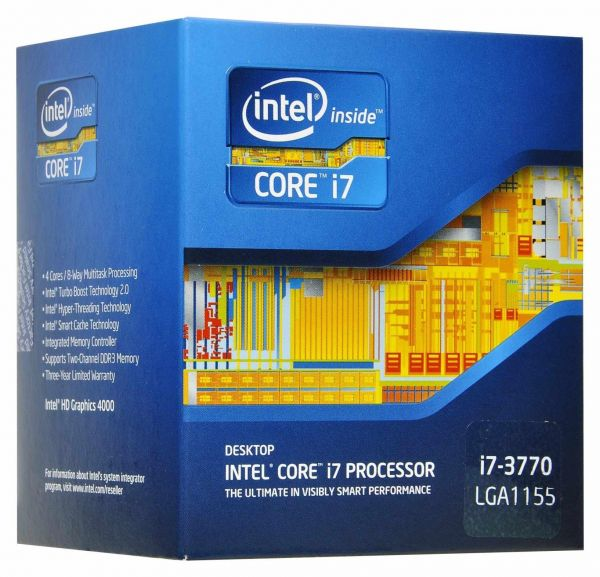
\includegraphics[width=7cm, keepaspectratio]{introduccion/intel_i7.jpg}
  %------------ TODO cite --------------%
  TODO cite imagen

  En cuanto al hardware, se realizó la comparación de tiempo de ejecución en el microprocesador Intel i7-3770\footnote{https://tinyurl.com/yb3tqpvu} con respecto a la tarjeta gráfica NVidia GTX 650 Ti\footnote{https://tinyurl.com/ycr3kouv}. Lo que representa una comparativa de trabajo simultáneo de 8 núcleos trabajando a 3.4GHz versus 768 núcleos trabajando a 928MHz para las operaciones pasibles a paralelismo.

  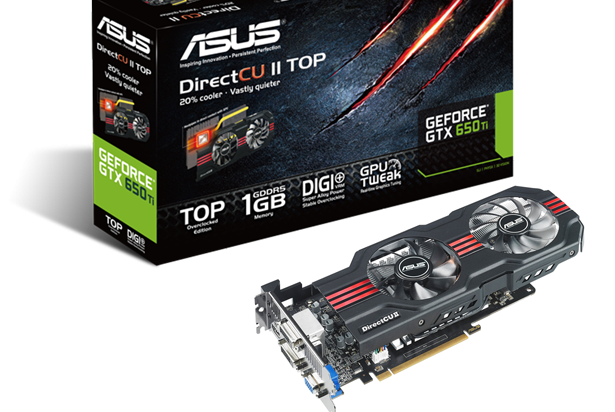
\includegraphics[width=12cm, keepaspectratio]{introduccion/gtx_650ti.png}
  %------------ TODO cite --------------%
  TODO cite imagen

  \bibliografia
\end{document}